In this section the methods used for determining appropriate control systems are explained. These systems should be able to keep the spacecraft on the trajectory as defined by the astrodynamics tool in section \ref{subsec:orbittool}. First the assumptions used and their effects on the accuracy of the analysis are explained in section \ref{control:assumptions}. Than, in section \ref{control:trim}, a point is determined in which the \gls{cg} should lie in order for the spacecraft to be trimmed at an angle of attack of *** as determined in section  \ref{subsec:orbittool}. The stability of the spacecraft is analysed in section \ref{control:stab}. In section \ref{control:system} the available control systems that can be used to follow the chosen angle of attack and bank angle profiles are weighed off.

\paragraph{Assumptions}
\label{control:assumptions}
**Primary and Secondary assumptions**

\paragraph{Trim point}
\label{control:trim}
The aerodynamic forces acting on the spacecraft work on the centre of pressure of the aeroshell. The \gls{cg} of the spacecraft has a certain offset in x,y and z direction with respect to this centre of pressure. Thus moments are induced around the center of gravity. These moments can be described as shown in equations \ref{eq:momx} - \ref{eq:momz}.
\begin{equation}
\label{eq:momx}
M_x = F_y \cdot dz - F_z \cdot dy
\end{equation}
\begin{equation}
\label{eq:momy}
M_y = F_x \cdot dz - F_z \cdot dx
\end{equation}
\begin{equation}
\label{eq:momz}
M_z = F_x \cdot dy - F_y \cdot dx
\end{equation}
Solving these equations such that $M_{x}$, $M_{y}$ and $M_{z}$ are zero results in figure \ref{}. From this figure it can be seen that the neutral location of the \gls{cg} 

\begin{figure}[h]
	\centering
	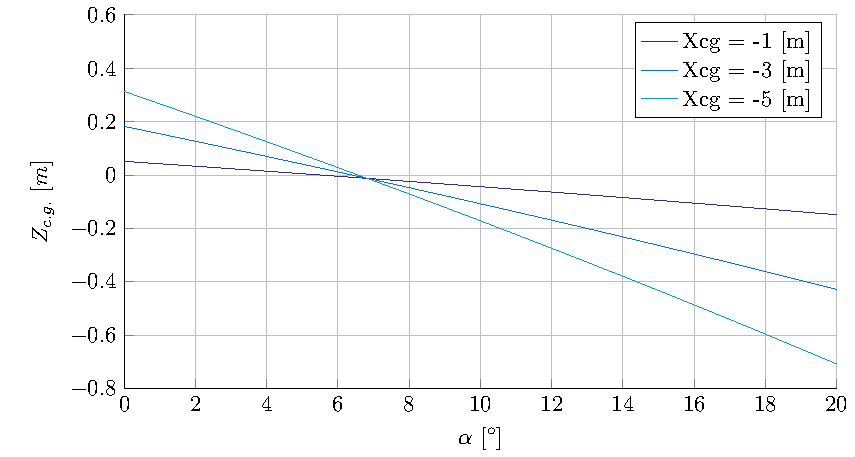
\includegraphics[width=0.8\textwidth]{./Figure/control/moment}
	\caption{1}
	\label{fig:}
\end{figure}
%\begin{figure}[h]
%	\centering
%	
\includegraphics[width=0.65\textwidth]{./Figure/Nyan}
%	\caption{nyan nyan om de X-as}
%	\label{fig:momx}
%\end{figure}
%\begin{figure}[h]
%	\centering
%	
\includegraphics[width=0.65\textwidth]{./Figure/Nyan}
%	\caption{nyan nyan om de Y-as}
%	\label{fig:momy}
%\end{figure}
%\begin{figure}[h]
%	\centering
%	
\includegraphics[width=0.65\textwidth]{./Figure/Nyan}
%	\caption{nyan nyan om de Z-as}
%	\label{fig:momz}
%\end{figure}

These equations result in a line in three-dimensional space for which the moments are 0 around each axis. This line is different for different combinations of forces which follow from different combinations of angle of attack, sideslip angle and bank angle.

\paragraph{Stability}
\label{control:stab}
The aerodynamic tool determines the static stability around all axis in the aerodynamic frame. If the spacecraft is stable around a certain axis all perturbations around that axis are automatically counteracted. However if an attitude change around that axis is required a larger moment has to be counteracted to control the spacecraft.  If the spacecraft is unstable around a certain axis perturbations around that axis have to be counteracted by active control. However if an attitude change around that axis is required a smaller moment has to be counteracted to control the spacecraft. It is thus preferred to perform control about the axis that are unstable and axis about which no control is needed are preferred to be stable.

\paragraph{Available control systems}
\label{control:system}
In this section three available control systems, a way of analysing their sizing and their application is explained. The control systems that are considered are \gls{cg} offset, thrusters and aerodynamic surfaces respectively.

\subparagraph{\acrlong{cg} offset}
In order to be able to trim the spacecraft at a certain angle of attack \gls{sym:alpha} a constant control moment has to be delivered by the combined control systems. To achieve this an active \gls{cg} offset control system is considered. By changing the location of the capsule \gls{cg} with respect to the aeroshell the magnitude of the resultant moments changes \cite{Mulqueen1991}. 
%This change can be computed with:
%\begin{equation}
%=
%\end{equation}

%From the stability analysis 

%**Not necessary for AoA, not feasible for bank**

\subparagraph{Thrusters}
\label{subpar:thrusters}
By dividing the required reaction control moment around a certain axis \gls{sym:Maero} with the length of the thruster moment arm \gls{sym:d} the required thruster control force $\gls{sym:F}_{req}$ can be determined. From the specific impulse of a thruster \gls{sym:Isp} and its propellant mass flow \gls{sym:mdot} follows the amount of thrust and control moment each thruster can generate \cite{Allen2012}:
\begin{multicols}{2}
\begin{equation}
\gls{sym:F}_{thrust}=\gls{sym:Isp}\gls{sym:ge}\gls{sym:mdot}
\label{eq:Fthrust}
\end{equation}
\begin{equation}
M_{control}=\gls{sym:F}_{thrust}\gls{sym:d}
\end{equation}
\end{multicols}
Where \gls{sym:ge} is the gravitational acceleration on earth. One can see from the preceding that for moment equilibrium $\gls{sym:F}_{req}=\gls{sym:F}_{thrust}$. By summing the thruster control force required over time the total propellant mass can be obtained. This relation is shown in Equation \ref{eq:mprop}.
\begin{equation}
m_{prop}=\int_{0}^{t} \frac{\gls{sym:F}_{thrust}}{\gls{sym:Isp}\gls{sym:ge}} dt = \int_{0}^{t} \frac{M_{control}}{\gls{sym:Isp}\gls{sym:ge}\gls{sym:d}} dt
\label{eq:mprop}
\end{equation}
Since a constant mass flow is needed to be able to deliver a continuous control moment thrusters are not considered to be used to trim the spacecraft at a certain angle of attack. Doing so would result in an excessively high propellant mass. \\
To arrive at a thruster design the specific impulse and maximum mass flow of available thrusters can be taken from literature. From this also follows the dry mass per thruster, which can be added to the propellant mass to arrive at the total thruster control system mass.

\subparagraph{Aerodynamic surfaces}
Using the modified Newtonian flow theory discussed in section \ref{subsec:aerotool} the force and moment contributions of a surface with a certain orientation to the freestream flow can be computed. For an aerodynamic surface (essentially a flap) the freestream inclination angle can be varied by using rotational actuators. Alternatively the flap area exposed to the freestream flow can be varied by using linear actuation. Both of these options directly influence \gls{sym:CD}\gls{sym:A} exerted on the actuated surface, thereby allowing active control.\\
The required control moments can be determined in a manner similar to section \ref{subpar:thrusters}. By comparing the required and delivered control moments the required force per flap can be computed. From this required force follows \gls{sym:CD}\gls{sym:A}. This depends on the flap area but also on the flap inclination angle. Using this \gls{sym:CD}\gls{sym:A} then forms the basis for computing the resultant flap drag corresponding to the aforementioned inclination angle.\\
An advantage of flaps is the possibility of having a low control system mass. This is possible because of the option to lock each flap in a certain orientation. This would require a minimum amount of power and would provide a stable source of control force coming from the aerodynamic forces exerted on it without requiring a constant mass flow, unlike thrusters.\\
This advantage poses a major disadvantage at the same time: No control force actuation is possible outside of the Martian atmosphere. Each time the spacecraft is not flying through the atmosphere and needs control actuation usage of the flaps is not possible. Thus thrusters would need to be used during these times, requiring additional mass.\\
A second disadvantage to using flaps comes from the option to lock the flap orientations. By doing this the weight can be kept low, but this also means a limited number of discrete flap settings would be available. This would make it hard to properly control the spacecraft by using these flaps, especially under the influence of disturbances.\\
A third complication of using flaps is the coupling between the force exerted by the flaps and the local structural deflection angle. The control force delivered by the flap causes the inflatable structure to deflect rearward, which causes the flap force to decrease. This in turn commences a decrease in structural deflection angle which will again increase the force exerted by the flaps. One can see from this that using flaps on the inflatable structure would induce oscillations in the spacecraft, whose effects on its stability and controllability are unknown.\\
Lastly, using body flaps on a non-winged re-entry vehicle has not yet been proven in flight. This poses a performance risk during concept development. This is in sharp contrast with the option of using thrusters as mentioned in section \ref{subpar:thrusters}. Thrusters have been used extensively and are the go-to option for ADCS' and as main propulsion system.